\chapter{Experiments}
\label{chapter:experiments}

This section describes, in detail, the methodology behind this dissertation's research objectives, namely:

\begin{itemize}
    \item Dataset description, preprocessing steps, and augmentation techniques;
    \item Experiments' descriptions, steps, settings, parameters, and conditions;
    \item Software stack used to describe said experiments in code;
    \item Computational resources used to execute the experiments.
\end{itemize}

Ultimately the experiments aim to study transfer learning in the specific domain of skin lesion classification, as well as compare its efficacy against simpler and more traditional learning schemes, by training and testing several models of different architectures and drawing helpful conclusions about the use of transfer learning techniques.

\section{Data}

The \ac{ISIC} 2017: Skin Lesion Analysis Towards Melanoma Detection grand challenge datasets \cite{isic2017} provides a training set with 2000 samples (divided into three classes: 374 melanoma, 254 seborrheic keratosis, and 1372 nevus), a validation set with 150 samples, and a test set with 600 samples. However training deep neural networks for skin lesion classification requires vast amounts of high quality, reliably labeled and verified data - a set of requirements which this dataset did not meet with confidence.

The \ac{HAM10000} \cite{ham10000} dataset is an effort to boost research on automated diagnosis of dermatoscopic images that focuses on the quality and reliability of the large volume of data that is so important for successful deep learning. The extracted images (where the lesion is centered if necessary) go through an extensive semi-automatic process that filters out non-dermoscopic imaging and unreliable diagnoses, after which they are submitted to a manual review to further confirm its quality.

The datasets from the \ac{ISIC} 2018 grand challenge \cite{isic2018} were largely based on \ac{HAM10000} that was already very high quality, which meant the data preprocessing needs would be much lower compared to the previous years' editions where all these quality guarantees had to be independently ensured by the competitors. The \ac{ISIC} 2018 datasets are therefore adequate for running these experiments.

\subsection{Preprocessing}
\label{subsection:preprocessing}

The images in the dataset undergo a number of preprocessing steps:

\begin{enumerate}
    \item Most readily available pretrained models are of network architectures whose input tensor is of square dimensions (e.g. $224 \times 224 \times 3$). Since our dataset's images are of distinct non-square dimensions, it is necessary to resize them to a square. However, resizing them all naively to the network's input tensor dimensions without regards to the image's aspect ratio means that the input fed to the network is of varying distinct aspect ratios which does not constitute a good start. Therefore, the first step is to crop an arbitrarily-sized square of the center of the image which will likely (and, in fact, does) capture the skin lesion.

    \begin{listing}[ht]
    \begin{minted}{python}
    def _crop(img):
        width, height = img.size
        if width == height:
            return img

        length = min(width, height)

        left = (width - length) // 2
        upper = (height - length) // 2
        right = left + length
        lower = upper + length

        box = (left, upper, right, lower)
        return img.crop(box)
    \end{minted}
    \caption{Function that crops a given image to a square crop of the center of the original image.}
    \label{code:crop}
    \end{listing}

\item Resize the images to the target networks' input dimensions $224 \times 224 \times 3$ and $299 \times 299 \times 3$. We resize them as soon as possible in the data pipeline in order to reduce the computational costs of any subsequent operations on the images.

    \begin{listing}[ht]
    \begin{minted}{python}
    def _resize(img, target_size):
        return img.resize(target_size, PIL.Image.NEAREST)
    \end{minted}
    \caption{Function that resizes a given image to the target dimensions.}
    \label{code:resize}
    \end{listing}

    \item Normalize the luminance and apply a 99\% contrast stretch to reduce the negative effect of changes in illumination and acquisition devices that alter the color of images \cite{colorconstancy}.

    \begin{listing}[ht]
    \begin{minted}{python}
    def _correct(img):
        img_y, img_b, img_r = img.convert('YCbCr').split()

        img_y_np = np.asarray(img_y).astype(float)

        img_y_np /= 255
        img_y_np -= img_y_np.mean()
        img_y_np /= img_y_np.std()
        scale = np.max([np.abs(np.percentile(img_y_np, 1.0)),
                        np.abs(np.percentile(img_y_np, 99.0))])
        img_y_np = img_y_np / scale
        img_y_np = np.clip(img_y_np, -1.0, 1.0)
        img_y_np = (img_y_np + 1.0) / 2.0

        img_y_np = (img_y_np * 255 + 0.5).astype(np.uint8)

        img_y = PIL.Image.fromarray(img_y_np)

        img_ybr = PIL.Image.merge('YCbCr', (img_y, img_b, img_r))
        return img_ybr.convert('RGB')
    \end{minted}
    \caption{Function that normalizes the luminance of an image and applies a 99\% contrast stretch.}
    \label{code:correct}
    \end{listing}
\end{enumerate}

\subsection{Augmentation}
\label{subsection:augmentation}

In our binary classification task (melanoma vs non-melanoma) the $m = 10015$ samples in the training set are highly imbalanced (illustrated in figure \ref{fig:classimbalance}):

\begin{itemize}
    \item the majority class has $|S_{maj}| = 8902$ samples, constituting $\frac{8902}{10015} \times 100 = 88.9\%$ of the samples;
    \item the minority class has $|S_{min}| = 1113$ samples, constituting $\frac{1113}{10015} \times 100 = 11.1\%$ of the samples.
\end{itemize}

\begin{figure}[ht]
    \centering
    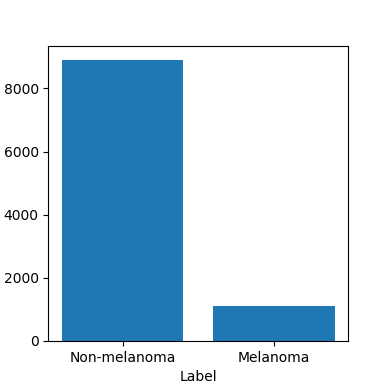
\includegraphics[width=0.5\textwidth]{figs/data_barplot.png}
    \caption{Bar plot of the distribution of the dataset's labels (melanoma or non-melanoma cases).}
    \label{fig:classimbalance}
\end{figure}

We correct this imbalance by oversampling the minority class, while also augmenting the total number of samples to $m' \approx 18000$ to increase the size of the dataset. That means we must augment the minority class by a factor of $\frac{\frac{m'}{2}}{|S_{min}|}$ and the majority class by a factor of $\frac{\frac{m'}{2}}{|S_{maj}|}$. For this augmentation we consider a set $T$ of possible transformations:

\begin{itemize}
    \item Horizontal flip
    \item Vertical flip
    \item 90º rotation
    \item 180º rotation
    \item 270º rotation
\end{itemize}

implemented by \verb|PIL.Image.transpose|\footnote{\url{https://pillow.readthedocs.io/en/stable/reference/Image.html\#PIL.Image.Image.transpose}} with the respective method:

\begin{itemize}
    \item \verb|PIL.Image.FLIP_LEFT_RIGHT|;
    \item \verb|PIL.Image.FLIP_TOP_BOTTOM|;
    \item \verb|PIL.Image.ROTATE_90|;
    \item \verb|PIL.Image.ROTATE_180|;
    \item \verb|PIL.Image.ROTATE_270|.
\end{itemize}

On principle, we did not consider transformations that change the color (e.g. contrast change, channel shift) or size (e.g. zoom) of features because it would unjustifiably allow the network to learn from these potentially misrepresenting features which even an expert human diagnosis would have trouble with.

The final available augmentations are all the $k$-combinations of the set $T$ for $k \in \{1, ..., |T|\}$, in other words all the possible ways in which you can combine the transformations from the set $T$.

\subsection{Split}

The number of variables in the future experiments would quickly lead to a combinatorial explosion of configurations, so to minimize the computational cost of the experiments a fixed validation scheme will be used rather than a cross validation scheme. To compensate for this lack of averaging over multiple folds of the data (which gives statistical confidence in the results), a fixed seed is set for every \ac{PRNG} as in code listing \ref{code:seed}, which in practice means parameters are initialized identically between experiments (providing some level of statistical confidence when making comparisons) and guarantees reproducibility.

\begin{listing}[ht]
\begin{minted}{python}
def seed():
    from random import seed
    seed(1)
    import numpy.random
    numpy.random.seed(2)
    from tensorflow import set_random_seed
    set_random_seed(3)
\end{minted}
\caption{Seed function that is called on every experiment to ensure reproducibility and similar conditions between experiments.}
\label{code:seed}
\end{listing}

The original training set from \ac{ISIC} 2018 is available for direct download, but the validation and test sets are kept private by the organization and are only used internally for reporting performance without actually releasing the data itself. As such, we will split the samples from the training set (which is available for download) into our own training, validation and test sets.

Augmentation, as described previously, results in 17810 samples which are split 85\%-15\% in a stratified fashion to maintain class balance within the splits into:

\begin{itemize}
    \item 15137 training samples, illustrated in figure \ref{fig:data_train};
    \item 2673 test samples, illustrated in figure \ref{fig:data_test}.
\end{itemize}

\begin{figure}[ht]
    \centering
    \includegraphics[width=0.6\textwidth]{../plots/data/train.png}
    \caption{Randomly-sampled images and respective labels of the train set.}
    \label{fig:data_train}
\end{figure}

\begin{figure}[ht]
    \centering
    \includegraphics[width=0.6\textwidth]{../plots/data/test.png}
    \caption{Randomly-sampled images and respective labels of the test set.}
    \label{fig:data_test}
\end{figure}

Since validation is intrinsically part of the training process itself, the validation set is a 15\% split from the training set obtained independently at the start of each training routine (also in a stratified fashion).

\section{Transfer Learning Experiments}

Based on the transfer learning techniques introduced in chapter \ref{chapter:background}, models of the VGG16 architecture pre-trained on ImageNet will be explored in order to repurpose the weights to a new model for skin lesion classification and draw conclusions about its efficacy.

It is hypothesized that

\begin{itemize}
    \item extracting features from lower layers of models trained for ImageNet classification can sometimes be better than higher layers, because the former presumably provide low-level features (e.g. shapesor lines) that are useful for skin lesion classification whereas the latter provide very high-level concepts (e.g. dogs, cats) that are relevant for classification in the ImageNet domain.
    \item extracting features from the last layer can sometimes be the most performant because optimization algorithms work globally on weights (which develop complex co-adaptations with other weights deep in the network), not on a per-layer basis, so it makes sense to extract all weights and fine-tune them to the target dataset.
\end{itemize}

To verify this, experiments based on this transfer learning approach will adhere to the following common methodology:

\begin{enumerate}
    \item Standardize training and validation samples relative to ImageNet;
    \item Some parameters are transfered from pre-trained models and otherwise initialized according to Xavier initialization;
    \item Define network architecture:
        \begin{enumerate}
            \item Extract features according to the specific experiment at hand;
            \item Use global average pooling to reduce the number of parameters before the classifier based on fully-connected layers;
            \item Stack fully-connected layers of ReLU-activated neurons;
            \item Add fully-connected layer with a single sigmoid-activated neuron for binary classification.
        \end{enumerate}
    \item Mini-batch \ac{SGD} with momentum $\gamma = 0.9$:
        \begin{itemize}
            \item Binary cross entropy cost function and explicit L2 regularization;
            \item 32 samples batches;
            \item Initial learning rate $\eta = 10^{-4}$ that decays by a factor of $10$ if the validation accuracy has not improved $+10^{-3}$ in the last $10$ epochs;
            \item Shuffle the $m$ samples every epoch;
            \item Train for a maximum of 1000 epochs, stopping early if the loss has not changed $\pm 10^{-3}$ in the last $30$ epochs.
        \end{itemize}
    \item Grid-search model selection based on the accuracy as measured on a fixed validation set;
    \item Final models will be evaluated and compared primarily using accuracy as measured on the test set.
\end{enumerate}

\subsection{VGG16}

% TODO: plot feature maps visualization
The basic unit in traditional \ac{CNN} architectures like VGG16 is the convolutional block, which is typically comprised by a number of convolutional layers and a pooling layer at the end to sum up the convolved features. These convolutional blocks are then stacked together in the hope to progressively build higher level feature maps at the end of each block. It is possible that the features at an arbitrary convolutional layer can be used for effective transfer learning, but in some sense it is expected that the features at a pooling layer are more relevant because that was the intended design. Not only that, but considering features at arbitrary convolutional layers originates a combinatorial explosion of possible feature extractions which is just not feasible given the computational resources. As such, we will only extract features at the end of each block (i.e. from pooling layers) because it is heuristically reasonable and significantly reduces the number of layers to extract features from.

% TODO: cartesian product notation math stuff
In the VGG16 architecture we are interested in extracting layers $e \in \{18,14,10,6,3\}$ and freezing layers $f \in \{18,14,10,6,3,0\}$ such that $e \geq f$ (because, obviously, one cannot freeze layers which were not extracted).

Additionally, for each of these settings, we grid-search the best $\lambda$ for L2-regularization from $\lambda \in \{10^{-10}, ..., 10^{2}\}$ (spaced evenly on a log scale). This yields a total of $200$ models, of which the top 10 are summarized in table \ref{table:vgg16_top10}.

Figure \ref{fig:vgg16_extract_freeze_study}, where $A_{test}$ is plotted against the number of extracted layers $e$ and the number of frozen layers $f$, shows that it is better to extract all $e = 18$ layers of features from the original model and fine-tune them, presumably because weights develop complex co-adaptations between them since optimization algorithms work globally and not on a per-layer basis.

\section{End-to-End Learning Experiments}

This section describes a set of experiments involving custom designed \ac{CNN} architectures whose models are trained from scratch, following the more traditional methodology typically called end-to-end learning, that will be used for comparison against the transfer learning approach which it is in direct contrast with.

These custom architectures are based around reasonable heuristics\footnote{\url{https://cs231n.github.io/convolutional-networks/}}:

% TODO: refactor, maybe this should go into background?
\begin{itemize}
    \item The most common form of a ConvNet architecture stacks a few CONV-RELU layers, follows them with POOL layers, and repeats this pattern until the image has been merged spatially to a small size. At some point, it is common to transition to fully-connected layers.
    \item Prefer a stack of small filter convolutional layers to one large receptive field convolutional layer
    \item It is very uncommon to see receptive field sizes for max pooling that are larger than 3 because the pooling is then too lossy and aggressive. This usually leads to worse performance.
    \item Reducing sizing headaches. The scheme presented above is pleasing because all the CONV layers preserve the spatial size of their input, while the POOL layers alone are in charge of down-sampling the volumes spatially. In an alternative scheme where we use strides greater than 1 or don’t zero-pad the input in CONV layers, we would have to very carefully keep track of the input volumes throughout the CNN architecture and make sure that all strides and filters “work out”, and that the ConvNet architecture is nicely and symmetrically wired.
    \item Why use stride of 1 in CONV? Smaller strides work better in practice. Additionally, as already mentioned stride 1 allows us to leave all spatial down-sampling to the POOL layers, with the CONV layers only transforming the input volume depth-wise.
    \item Why use padding? In addition to the aforementioned benefit of keeping the spatial sizes constant after CONV, doing this actually improves performance. If the CONV layers were to not zero-pad the inputs and only perform valid convolutions, then the size of the volumes would reduce by a small amount after each CONV, and the information at the borders would be “washed away” too quickly.
\end{itemize}

The experiments models of such architectures were trained from scratch as follows:

\begin{enumerate}
    \item Standardize training and validation samples relative to \ac{ISIC} 2018;
    \item Parameters are all initialized according to Xavier initialization;
    \item Define network architecture:
        \begin{enumerate}
            \item Stack blocks of convolutional and pooling layers to build useful features for classification;
            \item Use global average pooling to reduce the number of parameters before the classifier based on fully-connected layers;
            \item Stack fully-connected layers of ReLU-activated neurons;
            \item Add fully-connected layer with a single sigmoid-activated neuron for binary classification.
        \end{enumerate}
    \item Mini-batch \ac{SGD} with momentum $\gamma = 0.9$:
        \begin{itemize}
            \item Binary cross entropy cost function and explicit L2 regularization;
            \item 32 samples batches;
            \item Shuffle the $m$ samples every epoch;
            \item Initial learning rate $\eta = 10^{-4}$ that decays by a factor of $10$ if the validation accuracy has not improved $+10^{-3}$ in the last $10$ epochs;
            \item Train for a maximum of 1000 epochs, stopping early if the loss has not changed $\pm 10^{-3}$ in the last $30$ epochs.
        \end{itemize}
    \item Grid-search model selection based on the accuracy as measured on a fixed validation set;
    \item Final models will be evaluated and compared primarily using accuracy as measured on the test set.
\end{enumerate}

\subsection{Custom Architecture 1}

This custom architecture, illustrated in figure \ref{fig:custom1}, stacks three convolution-pooling blocks. Each block stacks two convolutional layers before the pooling layer, which is a good idea for large and deep networks because multiple stacked convolutional layers can develop more complex features of the input volume before the destructive pooling operation. Specifically,

\begin{enumerate}
    \item 32 filters, 3x3 kernel, 1x1 stride, same padding, ReLU activated
    \item 32 filters, 3x3 kernel, 1x1 stride, same padding, ReLU activated
    \item 2x2 max pooling
    \item 64 filters, 3x3 kernel, 1x1 stride, same padding, ReLU activated
    \item 64 filters, 3x3 kernel, 1x1 stride, same padding, ReLU activated
    \item 2x2 max pooling
    \item 128 filters, 3x3 kernel, 1x1 stride, same padding, ReLU activated
    \item 128 filters, 3x3 kernel, 1x1 stride, same padding, ReLU activated
\end{enumerate}

The classifier, illustrated in figure \ref{fig:custom1}, is a stack of two fully-connected layers of ReLU-activated neurons followed by a fully-connected sigmoid-activated neuron for binary classification.

\begin{enumerate}
    \item $u$ fully-connected ReLU-activated neurons;
    \item Another $u$ fully-connected ReLU-activated neurons;
    \item Single fully-connected sigmoid-activated neuron for binary classification.
\end{enumerate}

\begin{figure}[ht]
    \centering
    \includegraphics[width=1.0\textwidth]{figs/custom1.png}
    \caption{Architecture of the first custom-designed neural network.}
    \label{fig:custom1}
\end{figure}

We grid-search the best $\lambda$ for L2-regularization from $\lambda \in \{10^{-10}, ..., 10^{2}\}$ (spaced evenly on a log scale) as well as the number $u$ of ReLU-activated neurons in the antepenultimate and penultimate fully-connected layers from $u \in \{ 64, 128, 256, 512, 1024, 2048 \}$. This yields a total of $60$ models, of which the top 20 are summarized in table \ref{table:top20_custom1}.

\begin{table}[ht]
\centering
\begin{tabular}{ |c|c|c|c|c| }
\hline
$u$ & $\lambda$ & $A_{train}$ & $A_{val}$ & $A_{test}$ \\
\hline
128 & 1.61e-44 & 0.725 & 0.722 & 0.728 \\
256 & 1.27e-17 & 0.722 & 0.721 & 0.728 \\
256 & 3.29e-05 & 0.722 & 0.722 & 0.728 \\
256 & 1.74e-13 & 0.723 & 0.721 & 0.728 \\
256 & 7.88e-24 & 0.722 & 0.721 & 0.728 \\
64 & 3.04e-36 & 0.722 & 0.723 & 0.728 \\
256 & 1.17e-48 & 0.721 & 0.719 & 0.727 \\
256 & 2.21e-40 & 0.723 & 0.721 & 0.727 \\
256 & 2.4e-09 & 0.722 & 0.721 & 0.727 \\
64 & 2.59e-38 & 0.723 & 0.722 & 0.727 \\
64 & 1.61e-44 & 0.723 & 0.723 & 0.727 \\
64 & 1.89e-42 & 0.722 & 0.724 & 0.727 \\
64 & 6.72e-26 & 0.722 & 0.724 & 0.727 \\
128 & 1.08e-19 & 0.725 & 0.722 & 0.727 \\
256 & 1.08e-19 & 0.722 & 0.72 & 0.727 \\
256 & 1e-50 & 0.722 & 0.719 & 0.727 \\
256 & 9.24e-22 & 0.722 & 0.721 & 0.727 \\
64 & 1.27e-17 & 0.722 & 0.722 & 0.727 \\
64 & 2.21e-40 & 0.722 & 0.72 & 0.727 \\
64 & 3.29e-05 & 0.721 & 0.723 & 0.727 \\
\hline
\end{tabular}
\caption{Top 20 models of the custom architecture 1 sorted by $A_{test}$ in descending order.}
\label{table:top20_custom1}
\end{table}

The effect of $\lambda$ and $u$ on the performance of the model can be understood in figure \ref{fig:lambda_units_study_custom1}. As $u$ gets larger performance gets subtly but increasingly lower, so large $u$ is not worth it, especially when you consider the consequently larger number of parameters in the fully-connected layers which would have to be trained.

\begin{figure}[ht]
    \centering
    \includegraphics[width=0.5\textwidth]{../plots/plots_7/lambda_units_study/lambda_units_study.png}
    \caption{Accuracy of custom architecture 1 over a range of values for L2-regularization strength and the number of ReLU-activated neurons in the penultimate fully-connected layer.}
    \label{fig:lambda_units_study_custom1}
\end{figure}

\subsection{Custom Architecture 2}

This custom architecture, illustrated in figure \ref{fig:custom2}, stacks two convolution-pooling blocks. Each block uses a single convolutional layer before the pooling layer.

\begin{enumerate}
    \item 32 filters, 3x3 kernel, 1x1 stride, same padding, ReLU activated
    \item 2x2 max pooling
    \item 64 filters, 3x3 kernel, 1x1 stride, same padding, ReLU activated
    \item 2x2 max pooling
\end{enumerate}

The classifier is a single fully-connected layer of $u$ ReLU-activated neurons followed by a fully-connected sigmoid-activated neuron for binary classification.

\begin{enumerate}
    \item $u$ fully-connected ReLU-activated neurons;
    \item Single fully-connected sigmoid-activated neuron for binary classification.
\end{enumerate}

\begin{figure}[ht]
    \centering
    \includegraphics[width=1.0\textwidth]{figs/custom2.png}
    \caption{Custom Architecture 2}
    \label{fig:custom2}
\end{figure}

We grid-search the best $\lambda$ for L2-regularization from $\lambda \in \{10^{-10}, ..., 10^{2}\}$ (spaced evenly on a log scale) as well as the number $u$ of ReLU-activated neurons in the penultimate fully-connected layer from $u \in \{ 64, 128, 256, 512, 1024, 2048 \}$. This yields a total of $60$ models, of which the top 20 are summarized in table \ref{table:top20_custom2}.

\begin{table}[ht]
\centering
\begin{tabular}{ |c|c|c|c|c| }
\hline
$u$ & $\lambda$ & $A_{train}$ & $A_{val}$ & $A_{test}$ \\
\hline
64 & 1e-50 & 0.722 & 0.722 & 0.737 \\
64 & 0.452 & 0.656 & 0.657 & 0.651 \\
256 & 85300000.0 & 0.621 & 0.613 & 0.612 \\
512 & 9.24e-22 & 0.587 & 0.583 & 0.584 \\
256 & 1.74e-13 & 0.574 & 0.577 & 0.575 \\
512 & 53.0 & 0.567 & 0.58 & 0.558 \\
256 & 7.88e-24 & 0.56 & 0.544 & 0.553 \\
128 & 728000.0 & 0.556 & 0.559 & 0.547 \\
256 & 10000000000 & 0.544 & 0.54 & 0.534 \\
512 & 1.74e-13 & 0.537 & 0.522 & 0.534 \\
512 & 0.452 & 0.512 & 0.517 & 0.531 \\
128 & 3.04e-36 & 0.542 & 0.536 & 0.526 \\
64 & 2.81e-07 & 0.51 & 0.507 & 0.514 \\
1024 & 7.88e-24 & 0.496 & 0.5 & 0.504 \\
2048 & 2.04e-11 & 0.502 & 0.5 & 0.501 \\
1024 & 0.00386 & 0.5 & 0.5 & 0.5 \\
1024 & 1.49e-15 & 0.5 & 0.5 & 0.5 \\
1024 & 1e-50 & 0.5 & 0.5 & 0.5 \\
1024 & 2.4e-09 & 0.5 & 0.5 & 0.5 \\
1024 & 2.59e-38 & 0.5 & 0.5 & 0.5 \\
\hline
\end{tabular}
\caption{Top 20 models of the custom architecture 2 sorted by $A_{test}$ in descending order.}
\label{table:top20_custom2}
\end{table}

% TODO: citation needed

The effect of $\lambda$ and $u$ on the performance of the model can be understood in figure \ref{fig:lambda_units_study_custom2}. Since models of this architecture have much less parameters they are much less prone to overfitting, meaning that a wider range of values of $\lambda$ result in good performance.

\begin{figure}[ht]
    \centering
    \includegraphics[width=0.5\textwidth]{../plots/plots_2/lambda_units_study/lambda_units_study.png}
    \caption{Accuracy of custom architecture 2 over a range of values for L2-regularization strength.}
    \label{fig:lambda_units_study_custom2}
\end{figure}

\section{Hardware}

Initially, computational resources from \ac{IEETA} were used in very early exploratory research:

\begin{itemize}
    \item Intel® Xeon® Processor E5-2640;
    \item NVIDIA Tesla K40c;
    \item NVIDIA Quadro K4000;
    \item 32GB DDR4 RAM.
\end{itemize}

However, given that it was shared between dozens of other researchers it was deemed not enough for a comfortable and flexible workflow because:

\begin{itemize}
    \item the little amount of memory almost wasn't enough to load the dataset into memory, especially during critically busy times;
    \item the NVIDIA Quadro K4000, with a compute capability of 3.0, was unsupported by the software stack which required a minimum compute capability of 3.7, leaving only a single NVIDIA Tesla K40c to work with.
\end{itemize}

More recently, \ac{LAR}, located in the Department of Mechanical Engineering at the University of Aveiro, has provided access to their deep learning research server codenamed Deeplar:

\begin{figure}[ht]
    \centering
    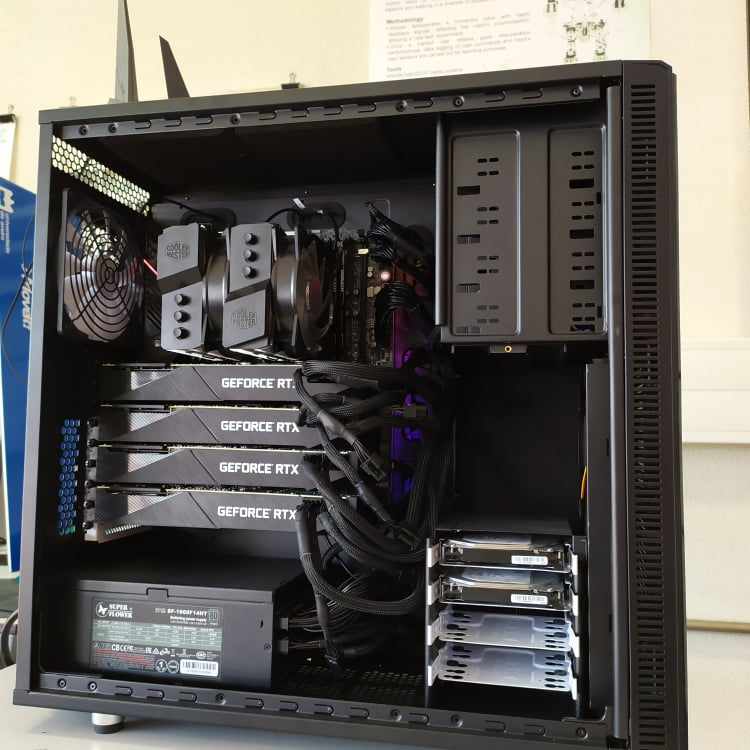
\includegraphics[width=0.4\textwidth]{figs/deeplar.jpg}
    \caption{Deeplar, the deep learning research server at \ac{LAR}}
    \label{fig:deeplar}
\end{figure}

\begin{itemize}
    \item AMD Ryzen™ Threadripper 2950X;
    \item Four NVIDIA GEFORCE® RTX 2080 Ti;
    \item 128GB DDR4 RAM.
\end{itemize}

The latter much more capable server (four state-of-the-art consumer \ac{GPU} and lots of \ac{RAM}) was effectively responsible for running this work's experiments.

\section{Software}

The deep learning research server Deeplar runs on openSUSE Tumbleweed 20191004\footnote{\url{https://software.opensuse.org/distributions/tumbleweed}}, a popular rolling-release GNU/Linux distribution. For interfacing with the \ac{GPU} it has installed CUDA 9.2 \footnote{\url{https://developer.nvidia.com/cuda-zone}} (NVIDIA GPU's proprietary language and API) and cuDNN 7.6.0 \footnote{\url{https://developer.nvidia.com/cudnn}} (a library for working with deep neural networks which most higher level frameworks rely on).

We used Miniconda\footnote{\url{https://docs.conda.io/en/latest/miniconda.html}} to install Conda\footnote{\url{https://conda.io/en/latest/}} which was used to manage a Python 3.6\footnote{\url{https://www.python.org/}} environment which was specifically required for compatibility with TensorFlow. Crucially, the following Python packages and specific versions were used for the development of most of the source code.

\begin{itemize}
    \item TensorFlow\footnote{\url{https://www.tensorflow.org/}} 1.12.0, of which we mostly use the \verb|tf.keras| API, for training and testing the various models;
    \item scikit-learn\footnote{\url{https://scikit-learn.org/}} 0.20.2 for some useful metrics and data splitting methods;
    \item NumPy\footnote{\url{https://numpy.org/}} 1.15.4 for various vector and matrix operations and Pillow\footnote{\url{https://pillow.readthedocs.io/en/stable/}} 5.4.1 for image handling and transformations because of this work's image preprocessing needs.
\end{itemize}
